% 图 13.1 —— 由 `checks/emit_hand.py` 自动拼出（probe 精测 + prims2 图元分解）
%%
% ⚠ 这是**稿子不是成品**：跑 `checks/checkhand.py 13.1` 看指标 + 看叠合图。
%%
%% ⚠ 待核：
%   · 本图 probe 报出阴影族 1 个 —— **本脚本不生成阴影**（要照原书手写）；prims2 的 strokes 里可能含阴影线，核对时留意别画重
%   · 可疑字形 1 项（空心圈 ⊙ 常被认成字母 o）—— 见文件末
%%
\documentclass[12pt]{standalone}
\usepackage{fontspec}
\setsansfont{Arial}
\newfontfamily\mfallback{DejaVu Sans}
\usepackage{tikz}
\begin{document}
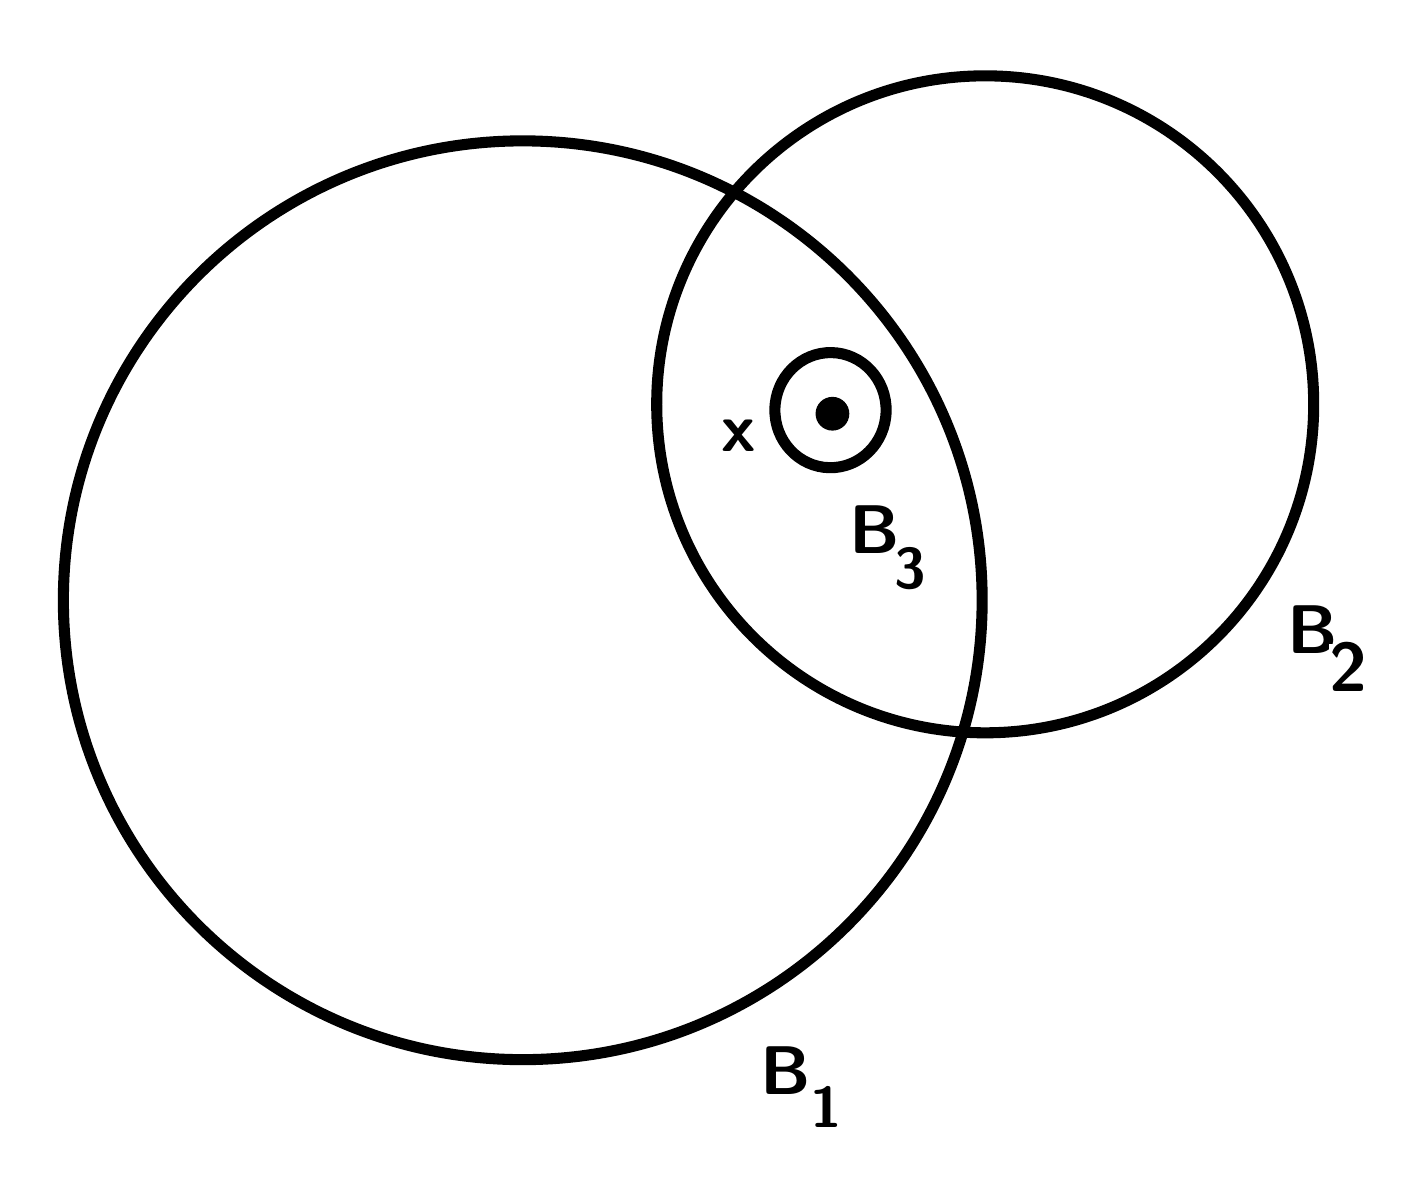
\begin{tikzpicture}[x=1pt, y=-1pt, line width=4.0pt, line cap=round, line join=round]

  %% ════ 填充区（prims2 的 fills）════

  %% ════ 圆 / 椭圆（probe 精测）════
  \draw (346.0,136.1) circle (118.7);
  \draw (178.9,206.9) circle (166.0);
  \draw[rotate around={178.9:(290.1,138.2)}] (290.1,138.2) ellipse (20.1 and 20.8);

  %% ════ 实心点 ════
  \fill (290.8,139.5) circle (6.1);

  %% ════ 标签（probe 直接给的 \node 行）════
  %% ⚠ 全部补了 fill=white：文字在最上层，否则与曲线交叉干扰
     \node[anchor=center,inner sep=0pt,fill=white,font=\fontsize{29.2}{36.5}\selectfont] at (257.0,147.4) {\textsf{\textbf{\textit{x}}}};   % box(248,137,16,17)
     \node[anchor=center,inner sep=0pt,fill=white,font=\fontsize{29.6}{37.0}\selectfont] at (306.2,181.5) {\textsf{\textbf{\textit{B}}}};   % box(295,170,19,22)
     \node[anchor=center,inner sep=0pt,fill=white,font=\fontsize{22.3}{27.9}\selectfont] at (318.9,195.6) {\textsf{\textbf{3}}};   % box(313,187,11,16)
     \node[anchor=center,inner sep=0pt,fill=white,font=\fontsize{29.6}{37.0}\selectfont] at (464.2,217.5) {\textsf{\textbf{\textit{B}}}};   % box(453,206,19,22)
     \node[anchor=center,inner sep=0pt,fill=white,font=\fontsize{22.9}{28.7}\selectfont] at (477.1,231.4) {\textsf{\textbf{2}}};   % box(471,223,11,16)
     \node[anchor=center,inner sep=0pt,fill=white,font=\fontsize{31.0}{38.8}\selectfont] at (273.8,377.0) {\textsf{\textbf{\textit{B}}}};   % box(262,365,20,23)
     \node[anchor=center,inner sep=0pt,fill=white,font=\fontsize{20.6}{25.7}\selectfont] at (288.4,390.3) {\textsf{\textbf{1}}};   % box(283,382,6,16)

  % 钉死画布：否则超出的图元/控制点会把页面撑大，1:1 回比就失准
  \pgfresetboundingbox
  \path[use as bounding box] (0,0) rectangle (491,408);
\end{tikzpicture}
\end{document}

% ⚠ 待核清单（probe 拿不准，人眼过一遍）：
%   · 未识别/跳过：⑤ 跳过/未识别的字形
